\documentclass[crop,class=article]{standalone}
%----------------------------Preamble-------------------------------%
\usepackage{tikz}                   % Drawing/graphing tools.
\usetikzlibrary{
    angles,                 % Drawing angles within triangles.
    quotes                  % Adding labels to angles.
}
%--------------------------Main Document----------------------------%
\begin{document}
    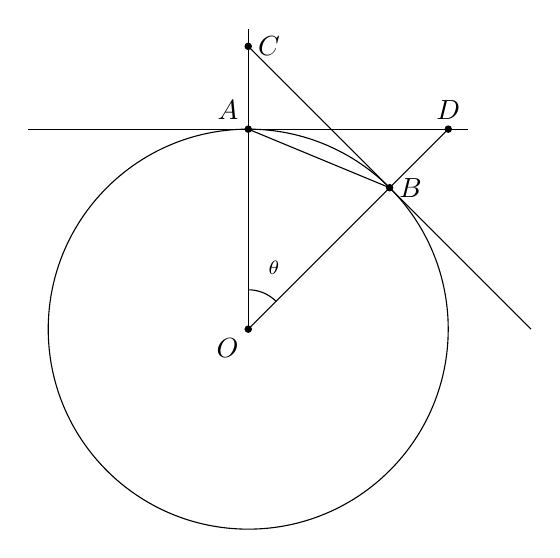
\begin{tikzpicture}
        \coordinate (O) at (0, 0);
        \coordinate (A) at (0, 1in);
        \coordinate (B) at (0.7071in, 0.7071in);
        \coordinate (C) at (0, 1.414in);
        \coordinate (D) at (1in, 1in);
        \coordinate (E) at (1.414in, 0);
        \draw (O) circle (1in);
        \draw (-1.1in, 1in) to (1.1in, 1in);
        \draw (O) to (0, 1.5in);
        \draw (A) to (B);
        \draw (O) to (D);
        \draw (C) to (E);
        \draw[fill=black] (O) circle (0.4mm);
        \draw[fill=black] (A) circle (0.4mm);
        \draw[fill=black] (B) circle (0.4mm);
        \draw[fill=black] (C) circle (0.4mm);
        \draw[fill=black] (D) circle (0.4mm);
        \node at (O) [below left] {$O$};
        \node at (A) [above left] {$A$};
        \node at (B) [right] {$B$};
        \node at (C) [right] {$C$};
        \node at (D) [above] {$D$};
        \pic[%
            draw=black,
            "\scriptsize{${\theta}$}",
            angle eccentricity=1.7,
            angle radius =0.5cm
        ]   {angle = D--O--C};
    \end{tikzpicture}
\end{document}